\section{Method}\label{sec:solution}

\subsection{Overview}
% We propose \textbf{\solutionTotalName{}} (\solutionSimpleName{}), which transforms time series forecasting into an image generation problem. First, the time series data is decomposed into trend components at three different time scales (short-term, medium-term, and long-term) and residuals using a moving average. Then, delay embedding and Short-Time Fourier Transform (STFT) are applied to convert these components into 2D images, which are subsequently fused into a unified image representation. Next, a diffusion model (EDM) is used to learn the distribution of future images, and future images are generated through denoising sampling. Finally, the generated images are transformed back into time series data through inverse transformations, and the individual trend components are reconstructed to obtain the final future predictions.

The proposed MR-CDM framework utilizes a five-stage pipeline to address multi-scale time series characteristics,as illustrated in \autoref{fig:architecture}. Initially, Multi-Scale Moving Average Decomposition (with windows of 5, 25, and 51) disentangles the input into short-term fluctuations, medium-term cycles, long-term trends, and high-frequency residuals~\cite{shen_multi-resolution_2024}. Subsequently, these components undergo domain transformation: delay embedding converts short- and medium-term signals into 32×32 images to preserve temporal dynamics, while STFT maps the long-term trend to the time-frequency domain to highlight periodicity. These representations are then concatenated into a 35-channel fused image. A conditional diffusion model~\cite{NEURIPS2020_4c5bcfec} then performs generation based on historical contexts to ensure temporal consistency. The process concludes with an Enhanced Hierarchical Reconstructor, which integrates hierarchical reconstruction, cross-scale attention, and adaptive weighting in parallel to recover high-fidelity predictions. This architecture effectively isolates multi-scale features, harnesses the generative power of diffusion models, and ensures precise detail recovery through multi-path fusion.

MR-CDM decomposes the input sequence into multi-scale components via a three-level moving average with window sizes of 5, 25, and 51, explicitly decoupling short-term fluctuations from seasonal periodicity. Trend1 and the residual, which carry local transient information, are mapped to image space~\cite{takens2006detecting,DBLP:conf/icassp/GriffinL83} via Delay Embedding to preserve fine-grained temporal dependencies. Trend3, representing long-term trends and seasonal cycles, is transformed via STFT to capture the amplitude and phase of periodic components in the time-frequency domain. Trend2 addresses medium-scale periodic structures between the two extremes. All four image branches are fused and modeled jointly by a diffusion model, followed by a hierarchical reconstructor to recover the predicted sequence. This branch-wise design prevents low-frequency components from masking high-frequency details, enhancing the model's ability to represent complex temporal dynamics.
\begin{figure*}[t]
    \centering           
    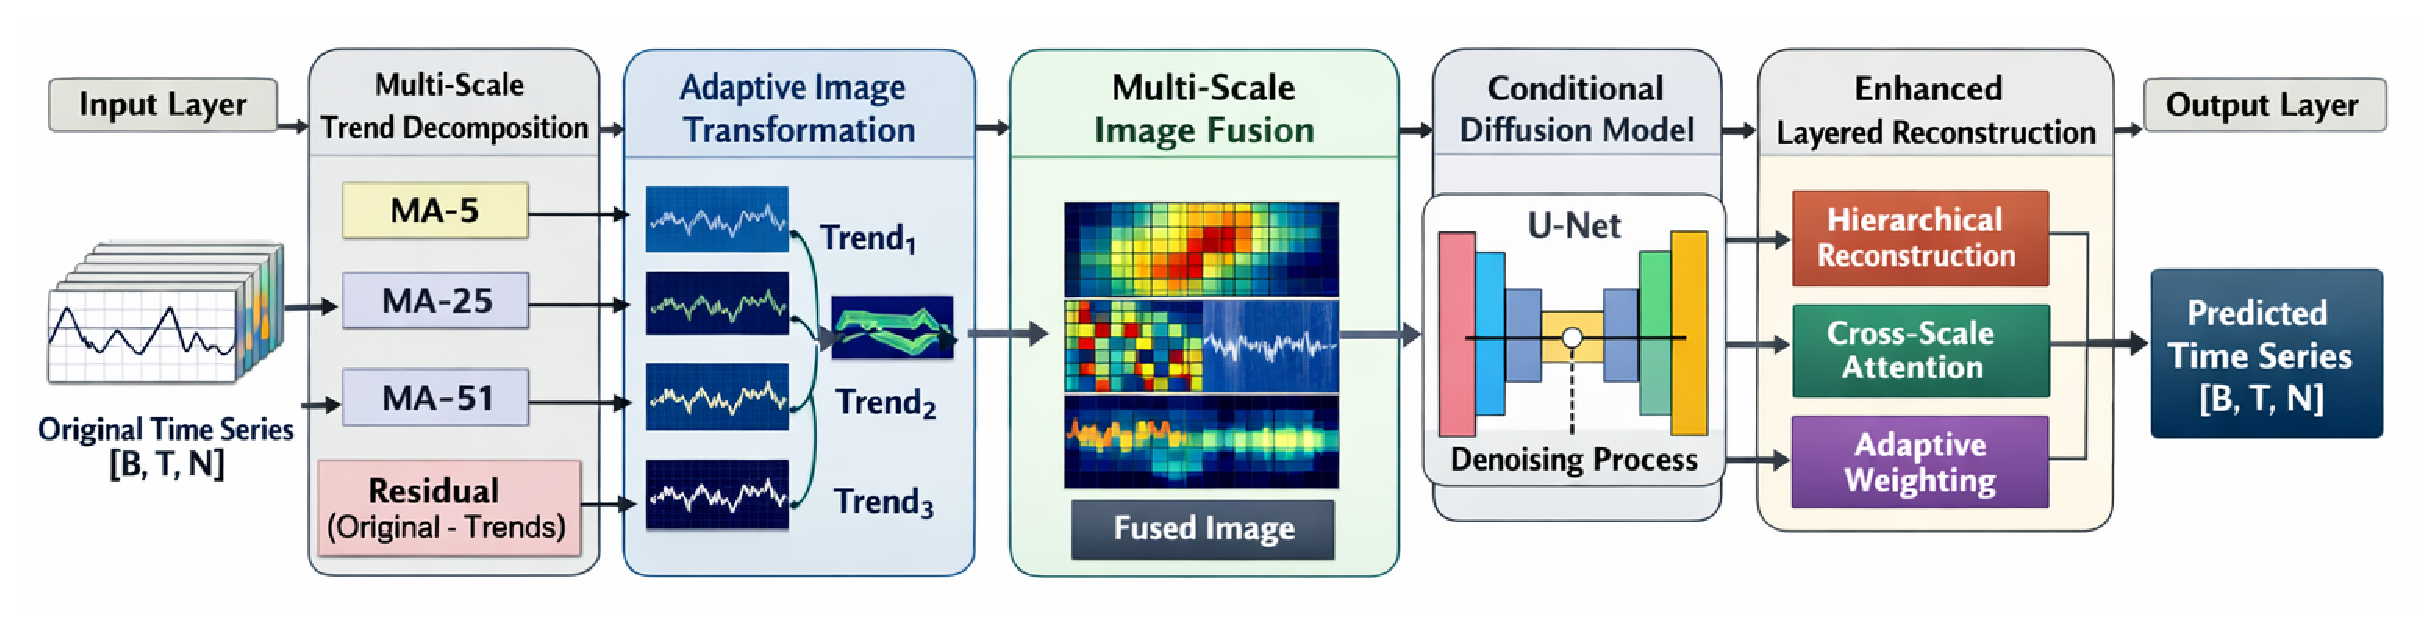
\includegraphics[width=0.8\textwidth]{figures/architecture2.eps}
    \caption{MR-CDM Model Architecture}
    \label{fig:architecture}
\end{figure*}

% \solutionSimpleName{} integrates three key innovations:
% \textit{Hierarchical Trend Decomposition.} The method decomposes time series data into short-term, medium-term, and long-term trend components, along with residuals, using moving averages. This multi-scale decomposition allows for the automatic extraction of varying temporal patterns across different time horizons.
% \textit{Time Series to Image Transformation.} By applying delay embedding and Short Time Fourier Transform (STFT), the decomposed trend components are transformed into 2D images, which are then fused into a unified image representation. This resolution-agnostic approach enables the flexible handling of time series data regardless of sequence length.
% \textit{Conditional Diffusion Model.} A diffusion model (EDM) is used to learn the distribution of future images, with the noise prediction network conditioned on both historical context and the extracted trend information. This enables the model to generate future time series through denoising sampling, ensuring accurate forecasting.



% \subsection{Hierarchical Trend Decomposition}
% Given three smoothing kernel sizes $\tau_1,\tau_2$ and $\tau_3$ with $\tau_1\leq\tau_2\leq\tau_3$, we apply \text{TrendExtraction} method by Equation~\eqref{eq:treand_extraction} to get the short-, medium- and long-term  trends, respectively.

% Algorithm~\ref{alg:htd} shows the process of Hierarchical Trend Decomposition.
% In Algorithm~\ref{alg:htd}, we apply \text{AvgPool(Padding($\cdot$))} from $\tau_1$ to $\tau_3$ to get different trends.
% At last, the residual $R$ is calculated by $X_0-X_1-X_2-X_3$.

% \begin{algorithm}[htbp]
% 	\DontPrintSemicolon
% 	\KwIn{time series segment $X_0$, smoothing kernel sizes $\tau_1,\tau_2$ and $\tau_3$}
% 	\KwOut{$X_1, X_2, X_3, R$}
% 	\caption{Hierarchical Trend Decomposition}
% 	\label{alg:htd}
% 	%\begin{algorithmic}[1]
% 	Initialize $R\gets X_0$\;
% 	\For{$s= 1$ \textbf{to} $3$} {
% 		$X_s\gets\text{AvgPool}(\text{Padding}(X_{s-1}), \tau_s)$\;
% 		$R\gets R-X_1-X_2-X_3$\;
% 	}
% 	\Return{$X_1, X_2, X_3, R$}\;
% 	%\end{algorithmic}
% \end{algorithm}

% \subsection{Resolution-Independent Input Transformation}
% After getting the short-, medium- and long-term trends as well as the residual, we apply adaptive delay embedding to transform the short-, medium-term trends and residual into 2-D image, we apply STFT to transform the long-term trend into 2-D image.
% Algorithm~\ref{alg:to_img} shows the process of Resolution-Independent Input Transformation.

% \begin{algorithm}[H]
% 	\DontPrintSemicolon
% 	\KwIn{short-term trend $X_1$, medium-term trend $X_2$, long-term trend $X_3$, residual $R$}
% 	\KwOut{trend images $\hat{X}_1,\hat{X}_2,\hat{X}_3,\hat{R}$}
% 	\caption{Resolution-Independent Input Transformation}
% 	\label{alg:to_img}
% 	%\begin{algorithmic}[1]
% 	$\hat{X}_1\gets\text{AdaptiveDelayEmbedding}(X_1)$\;
% 	$\hat{X}_2\gets\text{AdaptiveDelayEmbedding}(X_2)$\;
% 	$\hat{R}\gets\text{AdaptiveDelayEmbedding}(R)$\;
% 	$\hat{X}_3\gets\text{STFT}(X_3)$\;
% 	\Return{$X_1, X_2, X_3, R$}\;
% 	%\end{algorithmic}
% \end{algorithm}

% \subsection{Conditional Diffusion Process}
% The core innovation combines:

% \subsubsection{Multi-Scale Conditioning}
% The guidance signal $\mathbf{c}_s^t$ at level $s$ and timestep $t$ integrates:

% \begin{equation}
%     \mathbf{c}_s^t = \text{MLP}(\mathbf{z}_{\text{hist}}^s \oplus \widehat{\mathbf{Y}}_{s+1}^t)
% \end{equation}

% where:
% \begin{itemize}
%     \item $\mathbf{z}_{\text{hist}}^s = \text{TCN}(\mathbf{X}_s)$ (temporal convolutional network)
%     \item $\widehat{\mathbf{Y}}_{s+1}^t$ is the coarser-level prediction
%     \item $\oplus$ denotes channel-wise concatenation
% \end{itemize}

% \subsubsection{Adaptive Denoising}
% The noise prediction network $\epsilon_\theta$ implements:

% \begin{equation}
%     \epsilon_\theta^{(s)}(\mathbf{Y}_s^t, t, \mathbf{c}_s^t) = \text{U-Net}(\text{Conv1D}(\mathbf{Y}_s^t) \oplus \mathbf{E}(t) \oplus \mathbf{c}_s^t)
% \end{equation}

% with timestep embedding $\mathbf{E}(t)$ and U-Net architecture that maintains resolution-specific features.

% \subsection{Training and Inference}
% \subsubsection{Multi-Resolution Training}
% The joint optimization minimizes:

% \begin{equation}
%     \mathcal{L} = \sum_{s=1}^S \lambda_s \mathbb{E}_{t,\epsilon}[\|\epsilon - \epsilon_\theta^{(s)}(\mathbf{Y}_s^t, t, \mathbf{c}_s^t)\|_2^2]
% \end{equation}

% with resolution-specific weights $\lambda_s = 2^{s-S}$ emphasizing coarse levels.

% \subsubsection{Iterative Refinement Prediction}
% The inference process proceeds top-down:



% \subsection{System Properties}
% The complete framework provides:

% \begin{itemize}
%     \item \textbf{Resolution Flexibility}: Handles inputs with $L \in [64, \infty)$ through adaptive padding
%     \item \textbf{Multi-Scale Analysis}: Automatic decomposition into $S$ temporal scales
%     \begin{algorithm}[htbp]
% \caption{MR-CDM Prediction}
% %\begin{algorithmic}[1]
% Initialize $\widehat{\mathbf{Y}}_S^T \sim \mathcal{N}(0,\mathbf{I})$\;
% \For{$s = S$ \textbf{downto} $1$} {
% 	 \For{$t = T$ \textbf{downto} $1$}{
% 		$\widehat{\mathbf{Y}}_s^{t-1} = \alpha_t\widehat{\mathbf{Y}}_s^t + \sigma_t\epsilon_\theta^{(s)}(\widehat{\mathbf{Y}}_s^t,t,\mathbf{c}_s^t)$\;
% 	}
% 	\If{$s > 1$} {
% 		Upsample $\widehat{\mathbf{Y}}_s^0$ to initialize $\widehat{\mathbf{Y}}_{s-1}^T$\;
% 	}
% }
% \Return{$\mathcal{T}^{-1}(\widehat{\mathbf{Y}}_1^0)$}\;
% %\end{algorithmic}
% \end{algorithm}
%     \item \textbf{Conditional Uncertainty}: Diffusion process generates probabilistic forecasts
%     \item \textbf{End-to-End Training}: Joint optimization across all resolution levels
% \end{itemize}

% The architecture's modular design enables efficient computation through:
% \begin{equation}
%     \mathcal{C}(L) = O(S \cdot L \log L) \quad \text{FLOPs}
% \end{equation}
% making it scalable to long sequences while maintaining multi-resolution modeling capabilities.
\subsection{Proposed Algorithm}
The proposed MR-CDM framework follows a multi-stage pipeline detailed in prior work .We briefly summarize the core components here:

\textbf{Multi-Scale Decomposition:} Input time series are hierarchically decomposed into short, medium, and long-term trends using moving averages, alongside high-frequency residuals \cite{shen2024mr_diff}. 
\textbf{Time-Series-to-Image Mapping:} Temporal components are transformed into 2D image representations via adaptive delay embedding and STFT\cite{DBLP:journals/cssp/IshwaryaK25}, enabling resolution-independent processing. 
\textbf{Conditional Diffusion:} A multi-resolution diffusion process is employed, where noise prediction is conditioned on historical context and cross-scale features to ensure temporal consistency.